\documentclass{report}
\usepackage[english]{babel}

\usepackage[most,many,breakable]{tcolorbox}
\usepackage{xcolor}

\definecolor{defBoxBorder}{HTML}{395144}
\newtcolorbox{defBox}{colback=white,colframe=defBoxBorder,arc=3pt, boxrule=0.5pt, drop fuzzy shadow, title=Definition}
\definecolor{thBoxBorder}{HTML}{AC8441}
\newtcolorbox{thBox}{colback=white,colframe=thBoxBorder,arc=3pt, boxrule=0.5pt, drop fuzzy shadow, title=Theorem}
\definecolor{noteBoxBorder}{HTML}{4E6C50}
\newtcolorbox{noteBox}{colback=white,colframe=noteBoxBorder,arc=3pt, boxrule=0.5pt, drop fuzzy shadow, title=Note}
\definecolor{axBoxBorder}{HTML}{AA5656}
\newtcolorbox{axBox}{colback=white,colframe=axBoxBorder,arc=3pt, boxrule=0.5pt, drop fuzzy shadow, title=Axiom/Postulate}
\definecolor{corBoxBorder}{HTML}{8B7E74}
\newtcolorbox{corBox}{colback=white,colframe=corBoxBorder,arc=3pt, boxrule=0.5pt, drop fuzzy shadow, title=Corollary}
\definecolor{lemBoxBorder}{HTML}{B99B6B}
\newtcolorbox{lemBox}{colback=white,colframe=lemBoxBorder,arc=3pt, boxrule=0.5pt, drop fuzzy shadow, title=Lemma}


\usepackage[spanish]{babel}
\usepackage[utf8x]{inputenc}
\usepackage{amsmath}
\usepackage{graphicx}
\usepackage[colorinlistoftodos]{todonotes}
\usepackage{enumitem}
\usepackage{listings}
\usepackage{verbatim}
\usepackage{eurosym}
\usepackage[export]{adjustbox}
\usepackage{amssymb}
\usepackage{bussproofs}
\usepackage{amsmath}
\usepackage{tikz}
\usepackage{xcolor}
\usepackage{listings}
\usepackage{titletoc}
\usepackage{hyperref}

\hypersetup{
  colorlinks=true,
  linkcolor=black,
  urlcolor=blue,
  citecolor=black
}

\newcommand{\coverPage}[6]{%
%----------------------------------------------------------------------------------------
%	COVER START
%----------------------------------------------------------------------------------------
\begin{titlepage}

    \newcommand{\HRule}{\rule{\linewidth}{0.5mm}}
    \newcommand{\department}{#1}
    \newcommand{\course}{#2}
    \newcommand{\titleValue}{#3}
    \newcommand{\subtitleValue}{#4}
    \newcommand{\authorName}{#5}

    \center

    %----------------------------------------------------------------------------------------
    %	HEADER
    %----------------------------------------------------------------------------------------
    
\includegraphics{images/logo_usa.png}
    \vspace{0.5cm}
    \textsc{\Large \department}\\[0.5cm]
    \textsc{\Large \course}\\[0.5cm]
    \vfill

    %----------------------------------------------------------------------------------------
    %	TITLE
    %----------------------------------------------------------------------------------------

    \HRule\\
    \Huge
    \textbf{\titleValue}\\[0.5cm]
    \Large
    \textbf{\subtitleValue}\\
    \HRule\\[0.5cm]

    %----------------------------------------------------------------------------------------
    %	AUTHOR AND DATE
    %----------------------------------------------------------------------------------------

    \vfill
    \Large
    \textit{\authorName}\\
    {\large \today}\\[2cm]

\end{titlepage}
%----------------------------------------------------------------------------------------
%	COVER END
%----------------------------------------------------------------------------------------
}

\begin{document}
    \coverPage{ Mathematics }{ Integral Calculus and Series }{ Integrability }{  }{ Alexander Mendoza }{\today}
    \tableofcontents

    \chapter*{Prologue}
    After visiting the introductory course to infinitesimal Calculus, differential Calculus, we'll now continue with the course that will unleash the full potential of the derivative, Integral Calculus. In this first part of the course we'll begin by giving an intuitive idea of what the integral is, stating the problems that originated it. We will then formally define the integral of a function and state its properties to easily find its value. And we will finally provide the theorem that unifies differential and integral calculus, thus creating a relationship between the integral and the derivative of a function.

    \pagebreak
    \chapter{ Integrability }
    The main motivation of the integral was to have a way to calculate the area under some curve. For example, if you had a barrel without the bottom, you may want to know how much wood would you need to repair it. The first attempt known to tackle this problem was presented by Greek mathematicians, and was called the method of exhaustion. The method consisted of given a region, fill it up with a sequence of polynomial figures until filling up the area.

    \begin{Figure}
        \begin{center}
        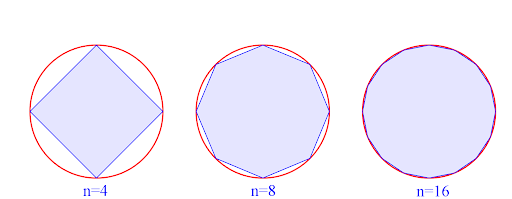
\includegraphics[width=1\textwidth]{images/exhaustion.png}
        \end{center}
    \end{Figure}

    Before formally defining the integral we will first need some definitions.
    \section{Inferior and Superior Sums}
    We will use both the superior and inferior sums to define the concept of an integral.

    \begin{defBox}
        \textit{\textbf{Partition of an integral.}} Let $a, b$ be real numbers such that $a<b$ and let $P$ be the following set

        $$P = \{x_0, x_1, \dots , x_n\}$$ with $a=x_0<x_1<\cdots<x_n=b$, then we say that $P$ is a partition of $[a,b]$
    \end{defBox}

    The concept of partition can be viewed simply as splitting the interval into smaller intervals and saving them inside a set.
    \begin{Figure}
        \begin{center}
            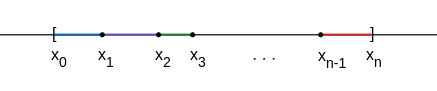
\includegraphics[width=1\textwidth]{images/partitions2.png}
        \end{center}
    \end{Figure}
    Figure 1.1.2 represents graphically the concept of a partition of an interval. Each colored part is a segment of the partition, and notice how the definition does not require the length of the segments to be equal.

    \begin{Example}
        Consider the interval $S = [-1, 6]$, then the set $\{0, \sqrt{2}, \frac{3}{2}, 4, 5\}$ would be a partition of $S$.
    \end{Example}
    \begin{defBox}
        \textit{\textbf{Minimum and maximum}}. Let $f$ be a function bounded on $[a,b]$ and let $P = \{x_0, x_1, \dots x_n\}$ be a partition of $[a,b]$. then

        The minimum of a function in $[a,b]$ is defined as
        $$m_i := inf\{f(x) | x_{i-1} \leq x \leq x_i\}$$
        And the maximum of a function in $[a,b]$ is defined as
        $$M_i := sup\{f(x) | x_{i-1} \leq x \leq x_i\}$$
    \end{defBox}

    % Add examples

    \begin{Example}
        Consider the function $$f(x) =
        \begin{cases}
        x^2 & \text{if } 0 \leq x < 1 \\
        1.5 & \text{if } 1 \leq x \leq 3 \\
        -1.5(x-5) & \text{if } 3 < x \leq 5
        \end{cases}$$
        Together with the interval $[0, 5]$ partition $P = \{\frac{1}{2}, \frac{3}{2}\}$

        \begin{center}
            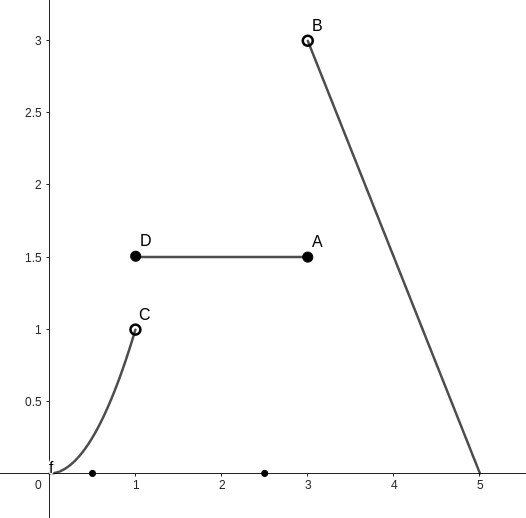
\includegraphics[width=.5\textwidth]{images/minmax.png}
        \end{center}

        Then the table of min an max values would be as follows

        \begin{center}
            \begin{table}[h]
                \begin{tabular}{l|l|l|l}
                $i$ & $[x_{i-1}, x_i]$             & $m_i$         & $M_i$         \\ \hline
                1   & $[0, \frac{1}{2}]$           & 0             & $\frac{1}{4}$ \\
                2   & $[\frac{1}{2}, \frac{5}{2}]$ & $\frac{1}{4}$ & $\frac{3}{2}$ \\
                3   & $[\frac{5}{2}, 5]$           & 0             & 3
                \end{tabular}
            \end{table}
        \end{center}

    \end{Example}

    With this we can now define the upper and lower sums.

    \begin{defBox}
        Suppose $f$ is bounded on $[a,b]$, let $P = \{t_0,\dots,t_n\}$ be a partition of $[a,b]$ and let

        $$m_i = inf\{f(x) | x_{i-1} \leq x \leq x_i\}$$
        $$M_i = sup\{f(x) | x_{i-1} \leq x \leq x_i\}$$

        Then we define the lower sum of $f$ for $P$, denoted by $L(f, P)$, as

        $$L(f, P) = \sum_{i=1}^{n}m_i(t_{i} - t_{i-1})$$

        and the upper sum of $f$ for $P$, denoted by $U(f, P)$, is defined as

        $$U(f, P) = \sum_{i=1}^{n}M_i(t_{i} - t_{i-1})$$
    \end{defBox}

    The lower and upper sums can be visualized as

    \begin{Figure}
        \begin{center}
        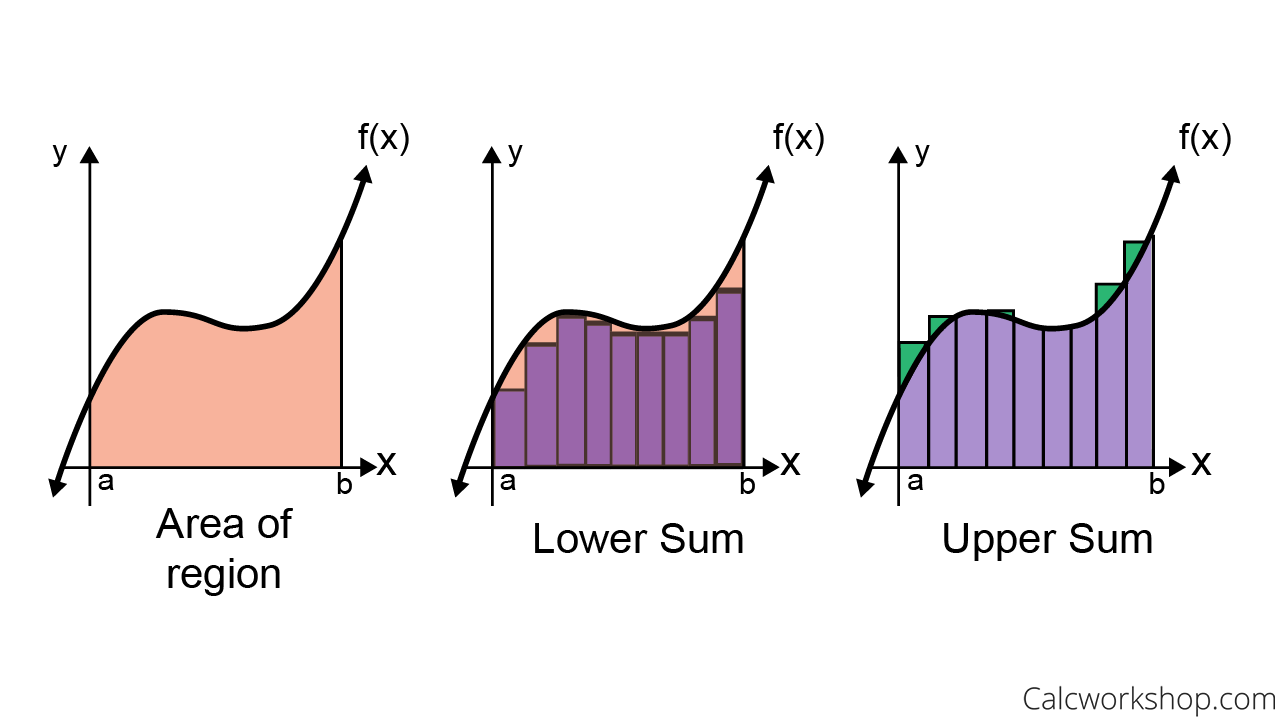
\includegraphics[width=1\textwidth]{images/lowerupper.png}
        \end{center}
    \end{Figure}

    \textbf{Function:} \( f(x) = x^2 \) over the interval \( [0, 2] \) with partition \( P = \{0, \frac{1}{2}, 1, \frac{3}{2}, 2\} \)

    \textbf{Lower Sum:}
    \[
    L(f, P) = 0 \times \frac{1}{2} + \frac{1}{4} \times \frac{1}{2} + 1 \times \frac{1}{2} + \frac{9}{4} \times \frac{1}{2} = 2
    \]

    \textbf{Upper Sum:}

    \[
    U(f, P) = \frac{1}{4} \times \frac{1}{2} + 1 \times \frac{1}{2} + \frac{9}{4} \times \frac{1}{2} + 4 \times \frac{1}{2} = \frac{17}{4}
    \]

    Let's now see which relation the lower and upper sum have. Our intuition may tell us that given $f$ bounded over $[a,b]$ and $P$ a partition of $[a,b]$, $L(f, P) \leq U(f, P)$, in fact this is true for any pair of distinct partitions. But, let's review first a lemma to demonstrate this fact.

    \begin{lemBox}
        Let $f$ be a bounded function and $P, Q$ be partitions of $[a,b]$. If $Q \subseteq P$, then

        $$L(f, Q) \leq L(f, P) $$
        $$U(f, P) \leq U(f, Q) $$
    \end{lemBox}

    \begin{ideaBox}
        The idea for this proof is to first demonstrate that the lemma is true for a partition $Q$ that contains only one more element than a partition $P$, and then construct a sequence of partitions, where each new partition will have one more element than the partition before it, and proof the general case.
    \end{ideaBox}

    \textit{\textbf{Proof.}}
    \noindent\textbf{First part of the proof}
    Let $f$ be a bounded function over $[a,b]$ and $P, Q$ be partitions of $[a,b]$ where $Q \subseteq P$ and $P$ contains only one more element than $Q$, namely $u$. We can represent $P$ and $Q$ as

    $$P = \{x_0,x_1,\dots,x_{k-1},x_k,\dots,x_n\}$$
    $$Q = \{x_0,x_1,\dots,x_{k-1},u,x_k,\dots,x_n\}$$

    Then let

    $$m' = inf\{f(x) | t_{k-1} \leq x \leq u\}$$
    $$m'' = inf\{f(x) | u \leq x \leq t_k\}$$

    And by definition of lower sum we have

    \begin{align*}
        L(f,P) &= \sum_{i=1}^{n} m_i(x_i-x_{i-1})\\
        &= \left(\sum_{i=1}^{k-1}m_i(x_i-x_{i-1})\right) \\
        &+ m_k(x_k-x_{k-1}) \\
        &+ \left(\sum_{i=k+1}^{n}m_i(x_i-x_{i-1})\right)
    \end{align*}

    Similarly

    \begin{align*}
        L(f,Q) &= \sum_{i=1}^{n} m_i(x_i-x_{i-1})\\
        &= \left(\sum_{i=1}^{k-1}m_i(x_i-x_{i-1})\right)\\
        &+ m'(u-x_{k-1}) + m''(x_k-u)\\
        &+ \left(\sum_{i=k+1}^{n}m_i(x_i-x_{i-1})\right)
    \end{align*}

    With this, it would be sufficient to show that $m_k(t_k-t_{k-1}) \leq m'(u - t_{k-1}) + m''(t_k-u)$. We know that $m_k \leq m'$, this because $\{f(x) | t_{k-1} \leq x \leq u\} \subseteq \{f(x) | t_{k-1} \leq x \leq t_k\}$ thus, this latter set contains all elements of the first set and it may contain smaller elements. A similar reasoning can be made to conclude $m_k \leq m''$. Then we have

    \begin{align*}
        m_k(t_k-t_{k-1}) &= m_k(t_k+0-t_{k-1})\\
        &= m_k(t_k+(-u+u)-t_{k-1})\\
        &= m_k((t_k-u)+(u-t_{k-1}))\\
        &= m_k(t_k-u)+m_k(u-t_{k-1})\\
        &\leq m''(t_k-u) + m'(u-t_{k-1}) &&\text{ This because inequality properties.}
    \end{align*}
    Therefore $L(f,P) \leq L(f, Q)$. The proof for the upper sum is analogous.\\

    \noindent\textbf{Second part of the proof}

    Suppose that $Q$ contains $m$ more points than $P$. Then we create a sequence of partitions for $[a,b]$, $\{P = P_0, P_1, P_2, \dots , P_m = Q\}$ where $P = P_0 \subseteq P_1 \subseteq P_2 \subseteq \dots \subseteq P_m = Q$ and $P_i$ contains one more point than $P{i-1}$, then by the first part of the proof

    $$L(f,P) \leq L(f,P_1) \leq L(f,P_2) \leq \cdots \leq L(f,Q)$$

    By transitivity, $L(f,P) \leq L(f,Q)$. Using a similar reasoning we have $U(f,P) \geq U(f,Q)$. Concluding our proof.
    \\

    Another useful observation goes as follows

    \begin{lemBox}
        Given any partition $P$
        $$L(f, P) \leq U(f, P)$$
    \end{lemBox}
    \textit{\textbf{Proof}}. We know this because
    $$L(f, P) = \sum_{i=1}^{n}m_i(t_{i} - t_{i-1})$$
    $$U(f, P) = \sum_{i=1}^{n}M_i(t_{i} - t_{i-1})$$
    and by definition, for any $i$:
    \begin{align*}
        m_i &\leq M_i\\
        m_i(t_{i} - t_{i-1}) &\leq M_i(t_{i} - t_{i-1})
    \end{align*}

    \begin{thBox}
        Let $P_1, P_2$ be partitions of an interval $[a,b]$ and let $f$ be bounded over $[a,b]$, then it's true that

        $$L(f, P_1) \leq U(f, P_2)$$
    \end{thBox}

    \textit{\textbf{Proof.}} Let $P = P_1 \cup P_2$, then by definition of union, $P_1 \subseteq P$ and $P_2 \subseteq P$, and by the previous lemma:

    $$L(f, P_1) \leq L(f, P)$$
    $$U(f, P) \leq U(f, P_2)$$
    By the afore mentioned observation, we have
    $$L(f, P) \leq U(f, P)$$
    And all together
    $$L(f, P_1) \leq L(f, P) \leq U(f, P) \leq U(f, P_2)$$
    Finally, by transitivity, we therefore have
    $$L(f, P_1) \leq U(f, P_2)$$
    Concluding our proof.\\

    With this we can state a theorem that will allow us to then define the integral of a function.
    \section*{The integral of a function}

    The formal definition of the integral is certainly complicated to provide. This can be noticed since we have already provided multiple definitions of things and sill haven't stated one for the integral. However, like all things in Mathematics, it's important to state concepts unambiguously, and it's not the exception with the integral. All this effort will be compensated, when we provide the fundamental theorem of calculus, reaching the full potential of the integral.

    We'll use the Darboux definition of the integral, which states as follows.

    \begin{defBox}
        Integral of a function. Let $f$ be a function bounded on $[a,b]$, $f$ is said to be integrable on $[a,b]$ if
        \begin{align*}
            \sup\{L(f,P) | P \text{ is a partition of } [a,b]\} \\
            = \inf\{U(f,P) | P \text{ is a partition of } [a,b]\}
        \end{align*}

        That common number is what we call the integral of $f$ over $[a,b]$ and is denoted by
        $$\int_{b}^{a}f$$

        And is read "the integral of $f$ over $[a,b]$"
    \end{defBox}

    This definition can be interpreted analytically as: whenever we have that the closest lower sum to the curve is equal to the closest upper sum to the curve, that common number is the integral. Graphically:

    \begin{Figure}
        \begin{center}
        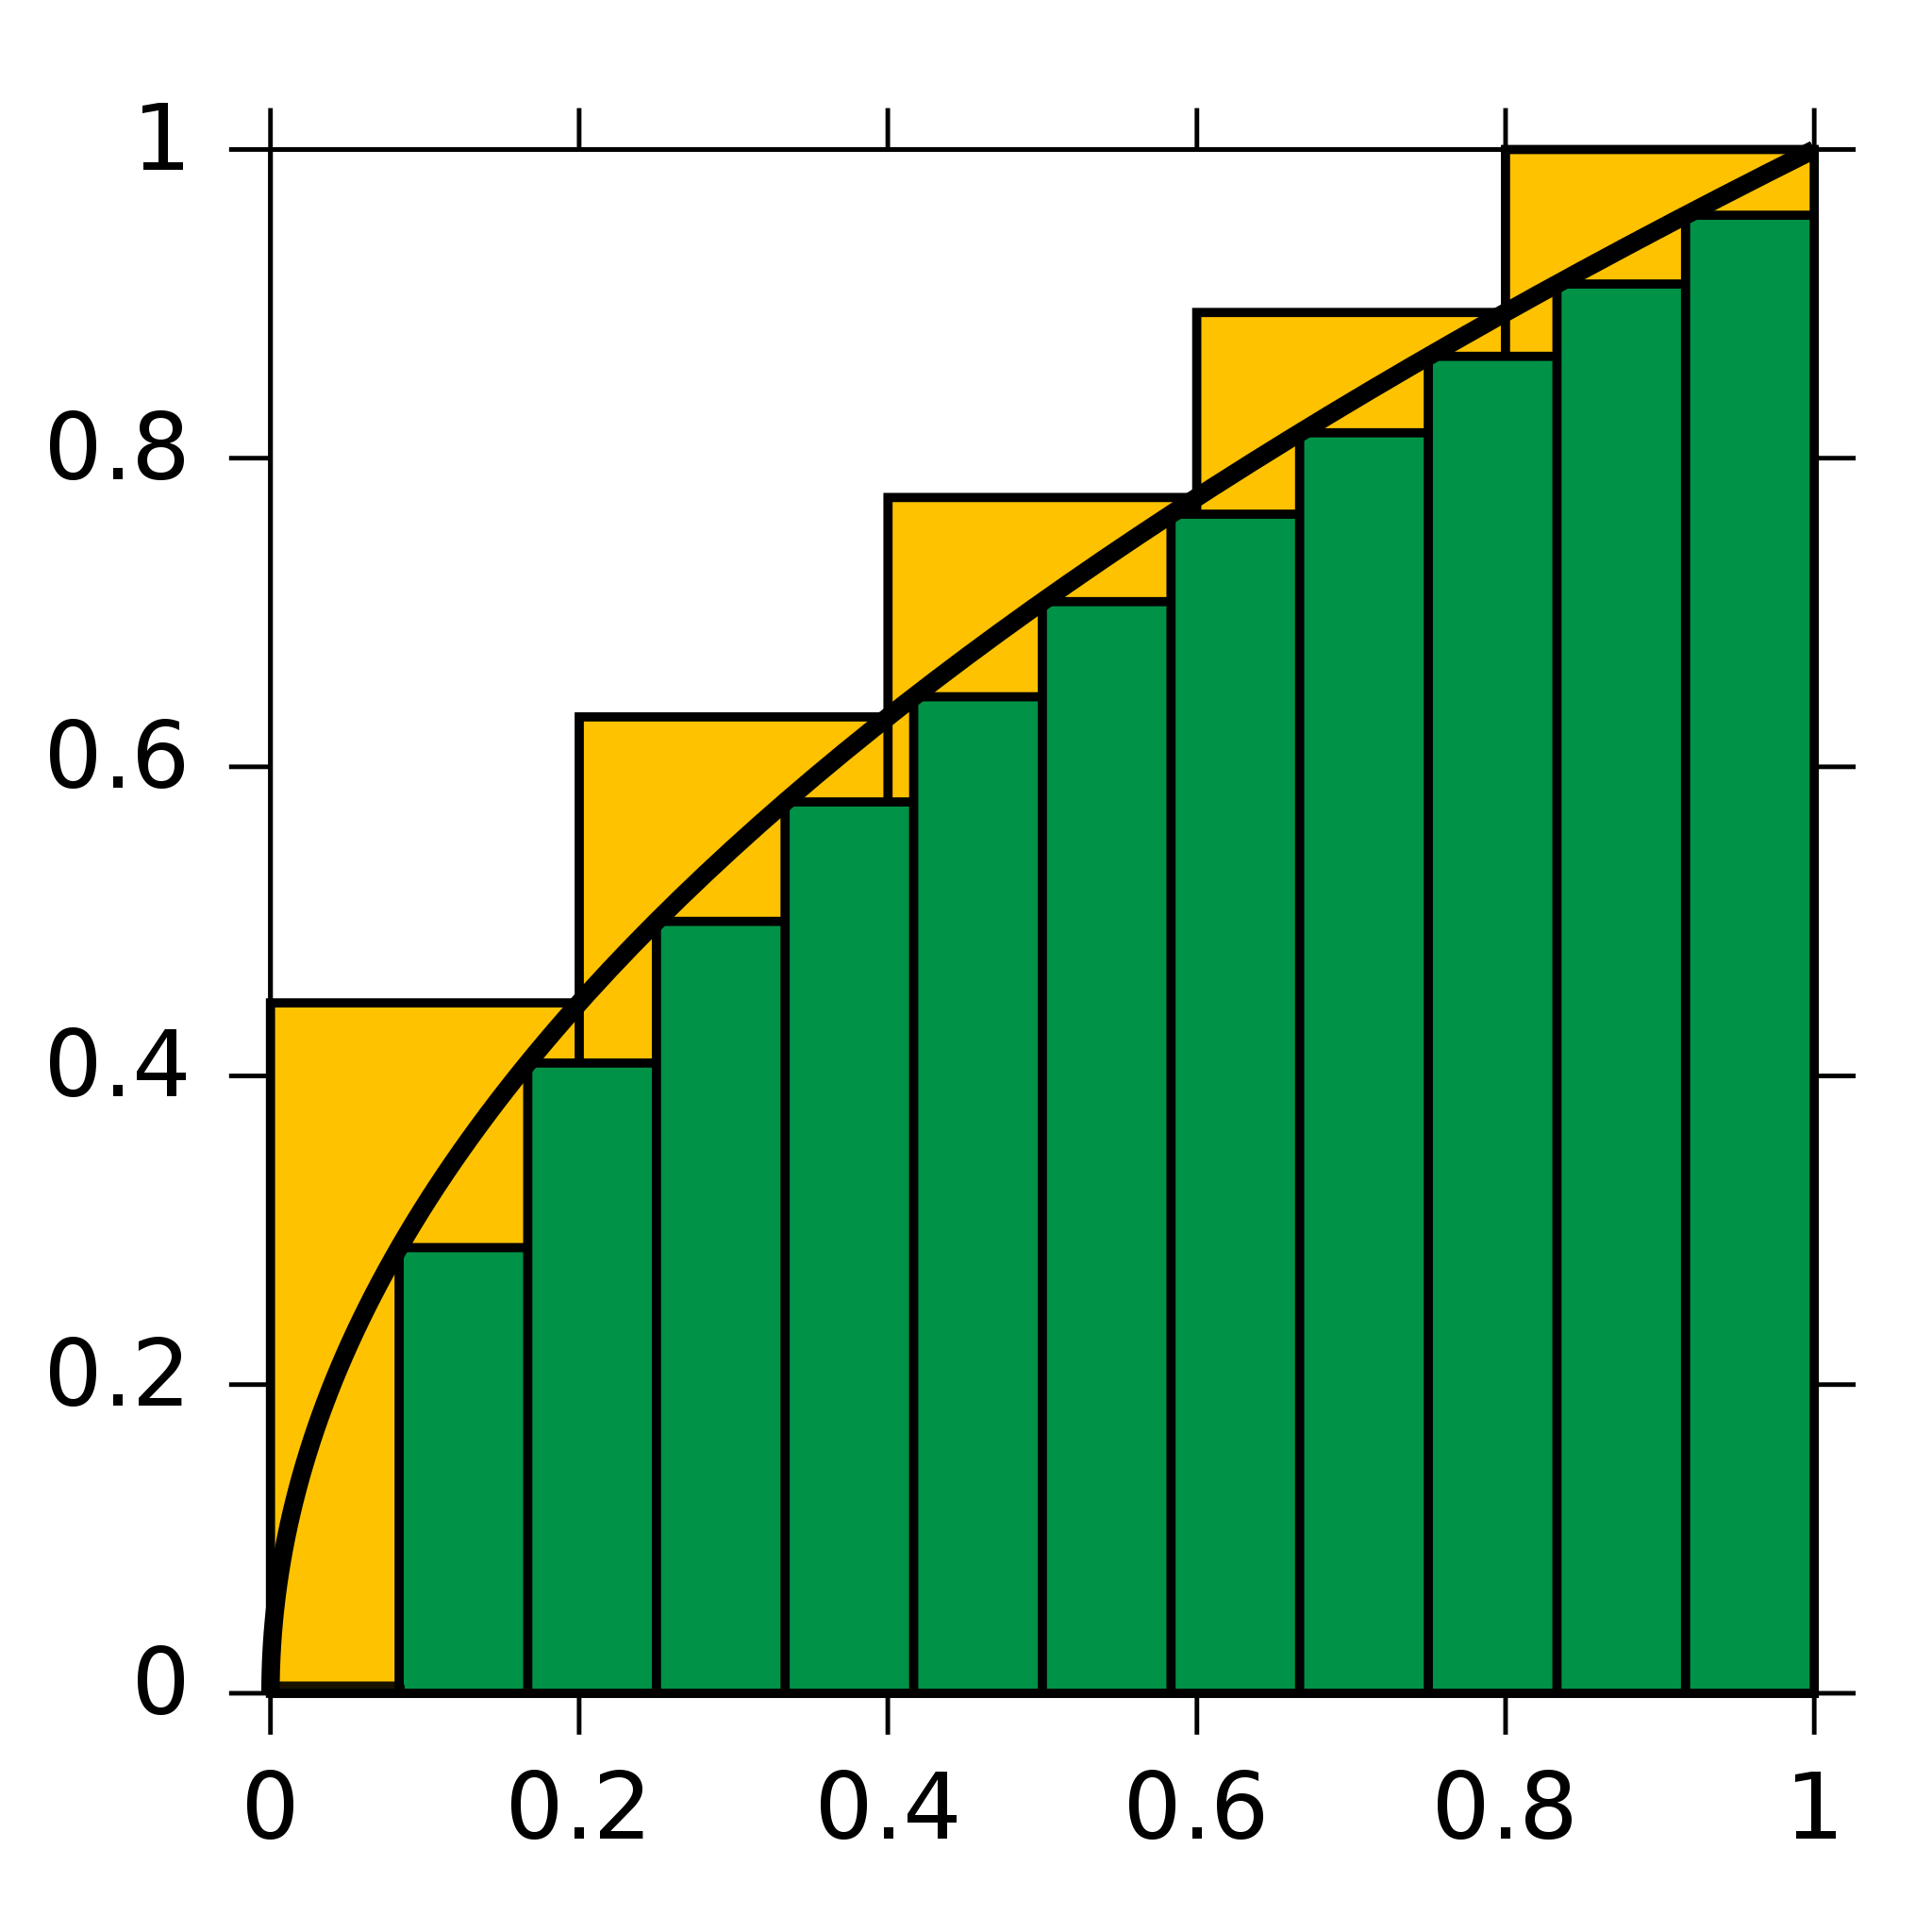
\includegraphics[width=.5\textwidth]{images/darbouxintegral.png}
        \end{center}
    \end{Figure}

    \begin{Example}
        Let $f(x) = C$ be a bounded function over $[a,b]$ for some constant $C$. Then $C = m_i = M_i$ for any partition $P$ in $[a,b]$. Then
        $L(f, P) = U(f, P) = C(b-a)$

        Thus, we have
        $$\sup\{L(f, P)\} = \inf\{U(f, P)\}$$

        Therefore, $f$ is integrable over $[a,b]$ and $\int_{b}^{a}f = C(b-a)$. Which would be the formula for a rectangle. Graphically:

        \begin{center}
            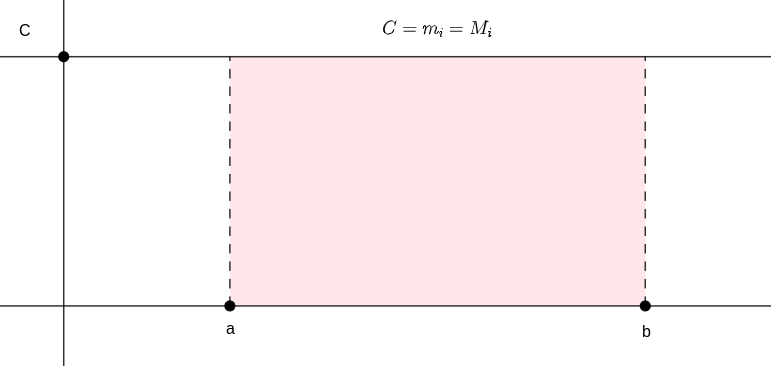
\includegraphics[width=1\textwidth]{images/integralconstant.png}
        \end{center}
    \end{Example}

    \begin{Example}
        Let $$f(x) =
        \begin{cases}
        1 & \text{if } x \text{ is rational} \\
        0 & \text{if } x \text{ is irrational}
        \end{cases}$$
        be a bounded function over the interval $[0,1]$

        We know that for any partition $P$, $m_i = 0$ and $M_i = 1$. Then
        $$ L(f, P) = 0 \neq U(f, P) = 1$$

        Thus
        $$\sup\{L(f, P)\} \neq \inf\{U(f, P)\}$$

        and therefore $f$ is not integrable over $[0,1]$.
    \end{Example}

    \section{Criterion for integrability}
    Now that we know how to know whether the integral of a function exists, we need an easier route to find the value of the integral.

    \begin{thBox}
        \textit{\textbf{Criterion for Integrability}}. If $f$ is bounded on $[a,b]$, then $f$ is integrable on $[a,b]$ if and only if, for every $\epsilon > 0$ there is a partition $P$ of $[a,b]$ such that
        $$U(f,P)- L(f,P) < \epsilon$$
    \end{thBox}

    \begin{noteBox}
        During the proof we'll use the fact that $a-b < \epsilon$ for any $\epsilon > 0$ implies that $a = b$. This can be checked using the archimedean property of the real numbers as follows:\\

        Suppose that $a \not = b$, then $a-b > 0$, by archimedean property, there exists n such that

        $$a-b > \frac{1}{n}$$

        This means that given $\epsilon = 1/n$, $a-b>\epsilon$, which contradicts our premise. Therefore $a=b$.
    \end{noteBox}

    \textit{\textbf{Proof.}} Let's start with the first implication of the proof. Suppose that for all $\epsilon > 0$, there exists $P$, partition of $[a,b]$, such that $U(f, P) - L(f, P) < \epsilon$ and let $\mathcal{P}$ be the set of all partitions of $[a,b]$, from this we get the following inequalities:
    \begin{align}
        \sup\{L(f, Q) | Q \in \mathcal{P}\} &\geq L(f,P)\\
        \inf\{U(f, Q) | Q \in \mathcal{P}\} &\leq U(f,P)
    \end{align}

    Multiplying the inequality 1.1 by $-1$ and add it to the inequality $1.2$ we get:
    $$
        \sup\{L(f, Q) | Q \in \mathcal{P}\} - \inf\{U(f, Q) | Q \in \mathcal{P}\} \leq U(f,P) - L(f,P)
    $$

    This implies:
    $$
        \sup\{L(f, Q) | Q \in \mathcal{P}\} - \inf\{U(f, Q) | Q \in \mathcal{P}\} < \epsilon
    $$

    And therefore $\sup\{L(f, Q) | Q \in \mathcal{P}\} = \inf\{U(f, Q) | Q \in \mathcal{P}\}$.\\

    Conversely, now suppose that $f$ is integrable over $[a,b]$, that is:
    $$\sup\{L(f, Q) | Q \in \mathcal{P}\} = \inf\{U(f, Q) | Q \in \mathcal{P}\}$$
    Then there exist $P', P'' \in \mathcal{P}$ such that $$U(f, P'') - L(f, P') < \epsilon$$ for all $\epsilon > 0$. If this is not true, we'll find a contradiction because of the supremum and infimum definitions.

    Now, let $P = P' \cup P''$, then by lemma 1.1.8 we have the following inequalities:
    \begin{align}
        L(f, P'') &\leq L(f, P)\\
        U(f, P') &\geq U(f, P)
    \end{align}
    And multiplying inequality 1.3 by $-1$ and adding it to inequality 1.4, we get
    $$U(f,P)-L(f, P) \leq U(f, P') - L(f, P'') < \epsilon$$

    And therefore, $U(f,P)-L(f, P) < \epsilon$.

    \begin{Example}
        Let $f(x) = x$ where $x \in [0,b]$, we then have that $m_i = x_{i-1}$ and that $M_i = x_i$. Then, by definition we know that:

        \begin{align*}
            L(f, P) &= \sum_{i=1}^{n} m_{i}(x_{i} - x_{i-1})\\
            &= \sum_{i=1}^{n}x_{i-1}(x_{i} - x_{i-1})
        \end{align*}
        And similarly:
        $$U(f, P) = \sum_{i=1}^{n}x_{i}(x_{i} - x_{i-1})$$

        Then

        \begin{align*}
            U(f, P)- L(f, P) &= \sum_{i=1}^{n} \left[x_i(x_i-x_{i-1}) - x_{i-1}(x_i-x_{i-1})\right]\\
            &= \sum_{i=1}^{n} \left[(x_i-x_{i-1})(x_i-x_{i-1})\right]\\
            &= \sum_{i=1}^{n} (x_i-x_{i-1})^2
        \end{align*}

        Now, let $P_n$ be partition of $[0,b]$ such that $x_i - x_{i-1} = \frac{b-a}{n} = \frac{b-0}{n} = \frac{b}{n}$, then:

        \begin{align*}
            U(f, P)- L(f, P) &= \sum_{i=1}^{n} \left(\frac{b}{n}\right)^2\\
            &= \frac{b^2}{n}
        \end{align*}

        Now, given $\epsilon > 0$ let $P_n$ be the previously defined partition of $[0,b]$ with $n > \frac{b^2}{\epsilon}$ in such a way that:

        $$U(f, P)- L(f, P) = \frac{b^2}{n} < \epsilon$$

        Therefore, $f$ is integrable.

        % COMPLETE THE PROOF FOR THE VALUE OF THE INTEGRAL
    \end{Example}

    % INSERT THE EXAMPLE FOR x^2

    \section{Uniform Continuity}

    We now shall define a concept that is going to help us to provide a theorem that will make our life easier to find whether a function is integrable or not.

    \begin{noteBox}
        Remember that the standard definition of continuity goes as follows:

        $f$ is continuous on a point $a$ if and only if, for all $\epsilon > 0$, there exists $\delta > 0$ in such a way that for all $x$, if $|x-a|<\delta$, then $|f(x) -f(a)| < \epsilon$.
    \end{noteBox}
    \begin{defBox}
        \textit{\textbf{Uniform continuity}}. $f$ is uniformly continuous over an interval $A$ if and only if, for all $\epsilon > 0$ there exists $\delta > 0$ in such a way that for all $x, y \in A$, if $|x-y| < \delta$, then $|f(x) - f(y)| < \epsilon$
    \end{defBox}

    This definition can be interpreted as follows, when small changes occur in $x$, they produce small changes in $f(x)$, but such changes on $f(x)$ do not depend of the value of $x$.

    % INSERT EXAMPLES FOR UNIFORM CONTINUITY

    Knowing this, we'll state some theorems that will help us prove that a continuous function is integrable.

    \begin{thBox}
        If $f$ is uniformly continuous over an interval $I$, then $f$ is continuous over $I$
    \end{thBox}

    \begin{thBox}
        \textit{\textbf{Heine-Cantor theorem}}. If $f$ is continuous over $[a,b]$ then $f$ is uniformly continuous over $[a,b]$
    \end{thBox}

    \begin{thBox}
        If $f$ is continuous over $[a,b]$, then $f$ is integrable over $[a,b]$
    \end{thBox}

    % COMPLETE THE PROOF

    \section{Algebra of integrals}

    So far we have stated some theoretical theorems, let's now review some operational ones.

    \begin{thBox}
        $f$ is integrable over $[a,b]$ if and only if, $f$ is integrable over $[a,c]$ and over $[c,b]$. Moreover:

        $$\int_{a}^{b}f = \int_{a}^{c}f + \int_{c}^{b}g$$
    \end{thBox}

    % \begin{ideaBox}
    %     The idea for the proof is to select a partition where one element of the partition is $c$, then create two more partitions one from 
    % \end{ideaBox}

    \textit{\textbf{Proof.}} Suppose that $f$ is integrable over $[a,b]$. Then 

    \begin{thBox}
        If $f$ and $g$ are integrable over $[a,b]$, then $f+g$ is integrable. Moreover:

        $$\int_{a}^{b}f+g = \int_{a}^{b}f + \int_{a}^{b}g$$
    \end{thBox}

    \begin{defBox}
        $$\int_{a}^{a}f = 0$$;
        $$\int_{a}^{b}f = - \int_{b}^{a}f \text{ if } a> b$$
    \end{defBox}

    \begin{thBox}
        If $f$ is integrable over $[a,b]$, then $c\cdot f$ is also integrable over $[a,b]$. Moreover:

        $$\int_{a}^{b}cf = c\cdot \int_{a}^{b}f$$
    \end{thBox}

    \begin{thBox}
        If $f$ is integrable over $[a,b]$ and $m\leq f(x) \leq M$ for all $x \in [a,b]$ then:

        $$m(b-a) \leq \int_{a}^{b}f \leq M(b-a)$$
    \end{thBox}

    % INSERT EXAMPLES ABOUT INTEGRABLE FUNCTIONS

    \section{The Fundamental Theorem of Calculus}

    After defining the integral, using a not very intuitive method; finding a criterion for integrability, which facilitates the process of finding integrable functions; proving that continuous functions are integrable; and lastly stating some properties of the integral, we'll now begin to construct our way to the most important theorem in all of Calculus, the fundamental theorem of calculus. This theorem will reveal the full potential of the integral and the derivative, unifying them together.

    \begin{thBox}
        If $f$ is integrable over $[a,b]$ and $F$ is defined on $[a,b]$ by $F(x) = \int_{a}^{x}f$, then $F$ is continuous over $[a,b]$.
    \end{thBox}

    % WRITE EXAMPLES

\end{document}
